In diesem Kapitel wird auf alle selbstkonstruierten Komponenten eingegangen, welche für die Messungen benötigt wurden. Zum einen gibt es eine Schuhkonstruktion, die es erlaubt, die in einer Gussform angefertigten MAP Sohlen einzuhängen, zum anderen wurde ein Laufsteg mit Rampenfunktion entworfen, welcher es erlaubt, Magnete unter die Lauffläche zu montieren. 

\subsection{Schuhkonstruktion} \label{Schuhkonstruktion}
\begin{figure}[tb]
	\hfill
	%\centering
	\begin{subfigure}[c]{.49\linewidth}
		\centering
		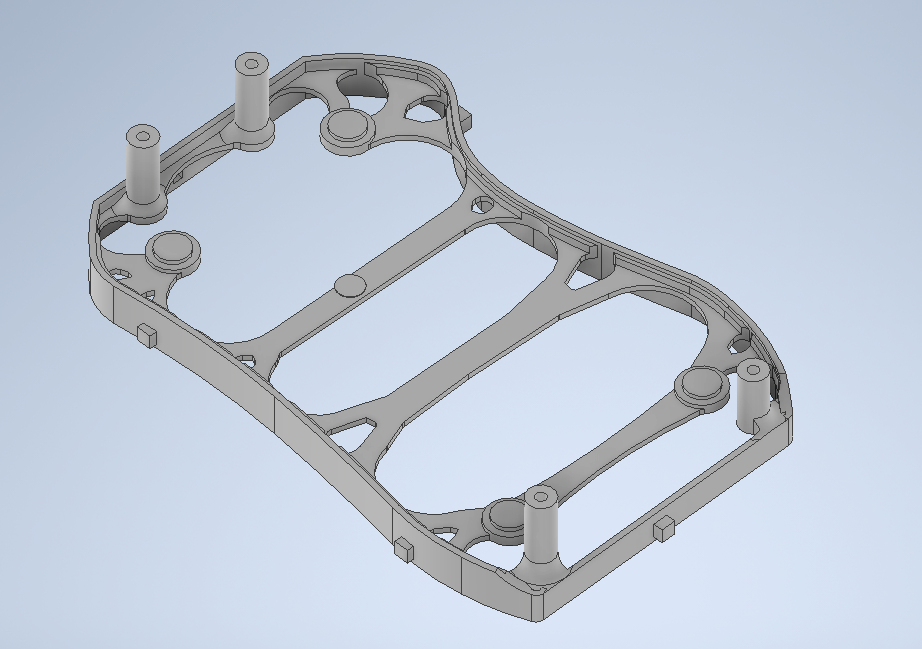
\includegraphics[width=\linewidth]{Bilder/Schuh_oben.png}
	\end{subfigure}
	\begin{subfigure}[c]{.49\linewidth}
		\centering
		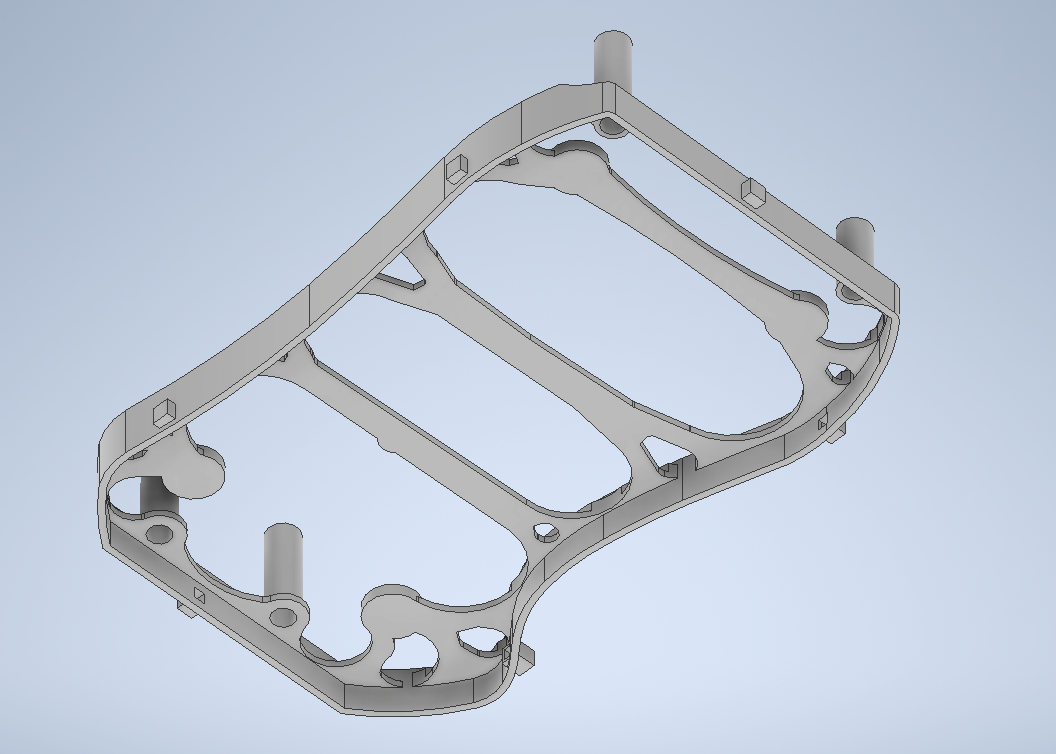
\includegraphics[width=\linewidth]{Bilder/Schuh_unten.png}
	\end{subfigure}
	\hfill
	\caption{Linker Schuh in Autodesk Inventors, Links von Oben, Rechts von Unten.}
	\label{Schuh_Inventor}
	%\vspace{0.1cm}
\end{figure}
Die Hülle eines Fußes von NAO besteht aus einem zweiteiligen Oberteil, welches das Fußgelenk abschließt und einem unteren Teil, welcher mit 4 Schrauben angebracht wird. Ohne Schraubenbefestigung liegt der Fuß nicht fest an. Die in Kapitel \ref{aufbau_NAO} beschriebenen vier Drucksensoren liegen dabei in dem unteren Teil auf Erhöhungen auf. Um die Auswirkungen anderer Sohlen für NAO messen zu können, muss der untere Teil des Fußes ausgetauscht werden. Dieser 	\glqq Schuh\grqq{} welcher die ursprüngliche Fußsohle ersetzt, enthält wiederum einen Steckplatz für die MAP Sohlen in verschiedenen Stärkegraden. 

In Abb. \ref{Schuh_Inventor} sind links die vier flachen Zylinder zu sehen, auf denen die Drucksensoren aufliegen. Die vier Zylinder an den Seiten sind die Führung der Schrauben, welche an das obere Teil des Fußes von NAO geschraubt werden. Die Außenform umschließt den oberen Teil während eine zweite Erhöhung, welche an den Innenseiten verläuft, auf dem Rand des oberen Teils aufsitzt, sodass die Passform fest ineinander greift. Da das gesamte Gewicht des NAO auf den 4 Drucksensoren lastet, kann Druckmaterial für die restliche Gesamtfläche bis auf stabilitätserhaltende Streben eingespaart werden. Diese Form wurde mit dem Shape Generator von Autodesk Inventor generiert, sodass sie längs bis zu einem $45^\circ$ Winkel ohne zu brechen gebogen werden kann. Die instabilsten Stellen sind die Zylinder der Schraubvorrichtung, welche durch Fillets verstärkt wurden. Diese Instabilität ist auf den schichtweise Druckvorgang durch das FDM Verfahren geschuldet und kann durch kleinere Schichthöhen ausgeglichen werden.

Die Unterseite, zu sehen in Abb. \ref{Schuh_Inventor} rechts, ist ein Hohlraum für die MAP Sohle zusammen mit den viereckigen Steckeinlässen für die Halterung. Die Seiten des Schuhs sind so hoch, dass das MAP etwa $1 \unit{mm}$ herausragt. Andernfalls würde NAO auf der Schuhkante laufen und nicht auf dem MAP.  
% wesentliche Aufgabe des Schuhs
% Stabiler Ersatz der vorherigen Sohle -> hält nur mit den Schrauben
% Druckverteilung auf die Sensoren 
% Einsparung von Material in der Mitte
% Anpassung an den oberen Teil durch Auflage und Umfassung
% Einfassung des MAPs
% Basiert auf dem Scan des zweiteiligen Fußes von NAO.
% 4 Schrauben befestigen den unteren Teil an das obere Teil. Der Schuh ersetzt die eigentliche Sohle
% Das Gewicht des Roboters lastet hauptsächlich auf den 4 Drucksensoren, welche in Kap (Theorie) bereits erklärt wurden. Die 4 kreisförmigen Flächen liegen deshalb genau da an, wo diese Sensoren auch in dem ursprünglichen Teil anlagen. 
% Shape generater tragende Oberfläche.

\subsection{Herstellung des MAP} \FloatBarrier
Der Herstellungsprozess allein dauert nicht mehr als eine halbe Stunde. Zunächst muss das Verhältnis für den Anteil des CIPs bestimmt werden. Die Masse ergibt sich aus
\begin{equation}
\text{m}_{\text{CIP}} = \frac{Ratio_{\text{CIP}} [\%]}{100\%}\cdot\text{m}_{ges},
\end{equation}
Die beiden additiven Komponenten A und B, welche auch als Basis und Katalysator bezeichnet werden, sind im Verhältnis 1:1 zu mischen. Das Volumen in \unit{ml} ergibt sich aus:
\begin{align}
\text{V}_\text{A} &= \frac{\text{m}_\text{A}}{\rho_\text{A}} ,& 
\text{V}_\text{B} &= \frac{\text{m}_\text{B}}{\rho_\text{B}}
\end{align}
mit $\rho_\text{A} = 1.071$ sowie $\rho_\text{B} = 1.046$ sowie
\begin{align}	
\text{m}_\text{A} &= \left( 1- \frac{Ratio_{\text{CIP}} [\%]}{100\%}\right)\times
\frac{\text{m}_{ges}}{\alpha + \beta}\times\alpha ,&
\text{m}_\text{B} &= \left( 1- \frac{Ratio_{\text{CIP}} [\%]}{100\%}\right)\times
\frac{\text{m}_{ges}}{\alpha + \beta}\times\beta,
\end{align}
Die Platzhalter $\alpha$ und $\beta$ stehen für das Mischverhältnis der jeweiligen Komponenten und sind hier Beide gleich 1, sodass die Formeln vereinfacht werden können in:
\begin{align}	
\text{m}_\text{A} &= \left( 1- \frac{Ratio_{\text{CIP}} [\%]}{100\%}\right)\times
\frac{\text{m}_{ges}}{2} ,&
\text{m}_\text{B} &= \left( 1- \frac{Ratio_{\text{CIP}} [\%]}{100\%}\right)\times
\frac{\text{m}_{ges}}{2}.
\end{align}

\begin{figure}[b]
	\hfill
	%\centering
	\begin{subfigure}[c]{.49\linewidth}
		\centering
		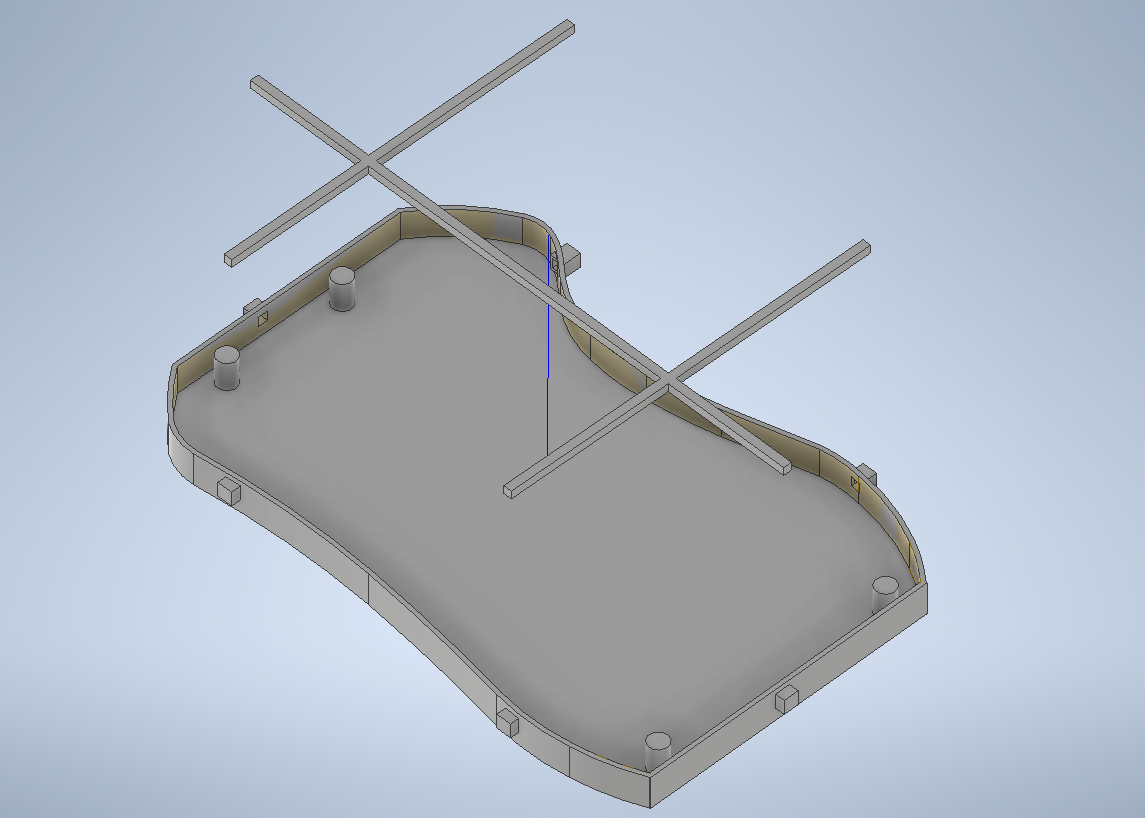
\includegraphics[width=\linewidth]{Bilder/Gussform_Innenteil_verschoben.png}
	\end{subfigure}
	\begin{subfigure}[c]{.49\linewidth}
		\centering
		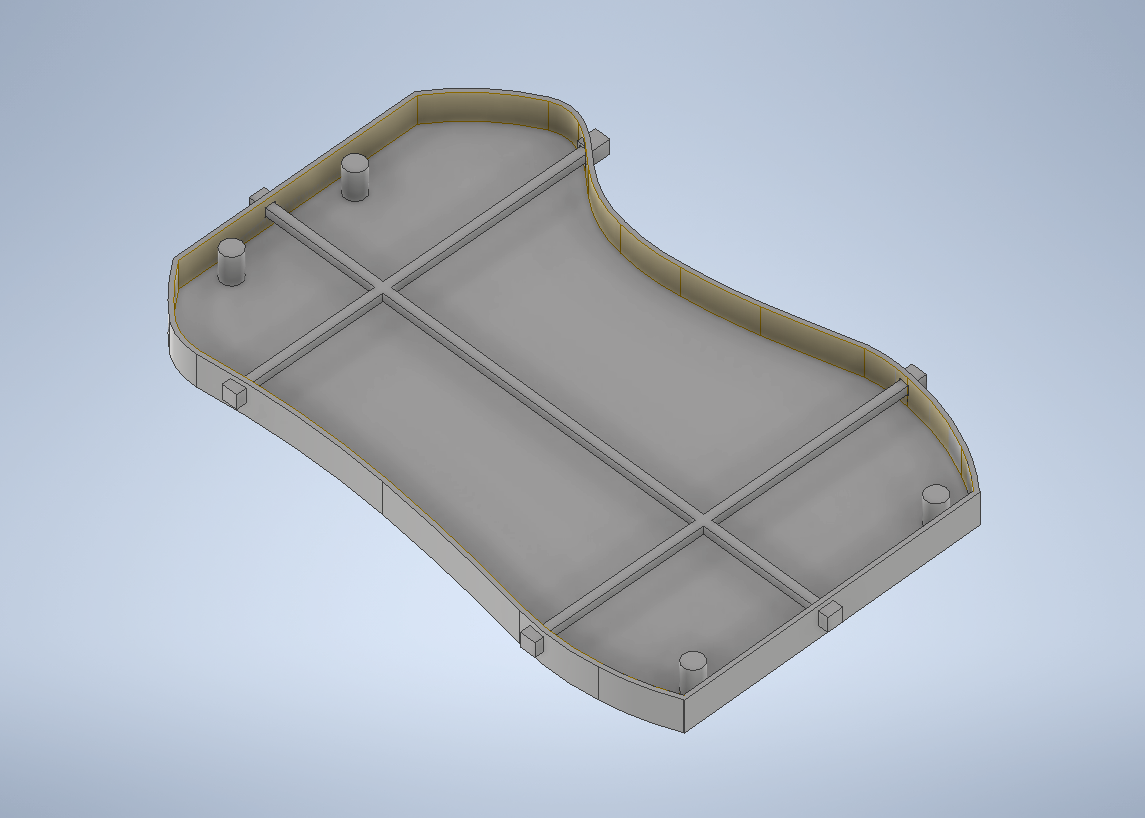
\includegraphics[width=\linewidth]{Bilder/Gussform.png}		
	\end{subfigure}
	\hfill
	\caption{Gussform der MAP Sohlen. Links ist die Innenhalterung herausgenommen, rechts ist sie eingespannt in den sechs Eckhalterungen.}
	\label{Gussform_Inventor}
	%\vspace{0.1cm}
\end{figure}

Mit der Laborwaage ABT 120-5DM von Kern wird $\text{m}_\text{CIP}$ in einem Becher abgemessen. Mit den Spritzen lassen sich $\text{V}_\text{A}$ und $\text{V}_\text{B}$ auf die ersten Nachkommastelle genau beifügen. Es handelt sich um SF13 2k-Silikon vom Hersteller Silikon Fabrik. Der Becherinhalt wird dann mit einem kleinen Mixstab gemischt, um eine gleichmäßige Verteilung der beiden Komponenten zu erreichen und somit eine optimale Vernetzung zu gewährleisten. Anschließend wird die Probe in einen Exsikkator gestellt, welcher mit einer Vakuumpumpe entgast wird, sodass das Silikon entgast ist. Schließlich kann das bis dahin noch flüssige MAP in die Gussform gegossen werden, nach spätestens einem Tag ist die Sohle dann komplett vernetzt. 

Da Silikon selbst sich nur sehr schlecht durch etwaige Klebstoffe nach der Vernetzung verkleben lässt wird hier wie in Abb. \ref{Gussform_Inventor} zu sehen ist, eine $2\unit{mm}$ dicke Stangenkonstruktion eingehängt, welche bis auf die 6 Enden mit MAP umschlossen wird. Dieses aus PLA gedruckte Konstrukt ist flexibel und kann deshalb durch Verbiegen in die Verankerungen gedrückt werden. Nach der vollständigen Vernetzung kann die Sohle aus der Form entnommen und in den Schuh aus dem vorherigen Kapitel eingesetzt werden. 

Die vier Zylinder dienen als Platzhalter um die sechs Ecken in der Halterung des Schuhs für einen besseren Halt festzukleben und dann durch die Löcher des MAPs die Schrauben lockern zu können. 

Das Silikon selbst hat eine zu große Haftung, v.a. durch die Fläche des Schuhs. Deshalb wird es vor der Messung mit Speisestärke eingedeckt, was eine Bodenhaftung ähnlich der Plastiksohle des Originalschuhs von NAO zur Folge hat. Dies verhindert außerdem ungewollte Adhäsion.

\subsection{Laufstegkonstruktion} \FloatBarrier

Der NAO Roboter ist für den Einsatz auf geraden Bodenflächen im Innenbereich ausgelegt wobei er bei einem Bewegungsablauf ohne Anpassung an die Umwelt wie mit dem Befehl \texttt{moveTo()} durch Rutschen nicht immer die gleiche Strecke zurücklegt. 
Um wiederholbare Messreihen garantieren zu können ist eine Teststrecke von Nöten. Des Weiteren sind verschiedene, flache Untergründe für eine Sohlenentwicklung interessant.
\begin{figure}[hb]
	\hfill
	%\centering
	\begin{subfigure}[c]{.49\linewidth}
		\centering
		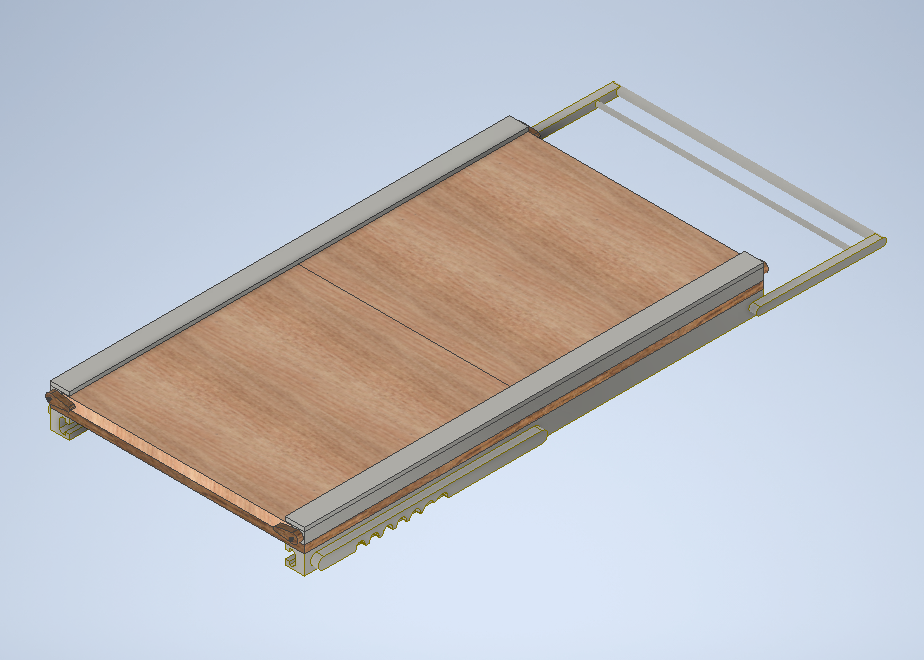
\includegraphics[width=\linewidth]{Bilder/Rampe_oben.png}
	\end{subfigure}
	\begin{subfigure}[c]{.49\linewidth}
		\centering
		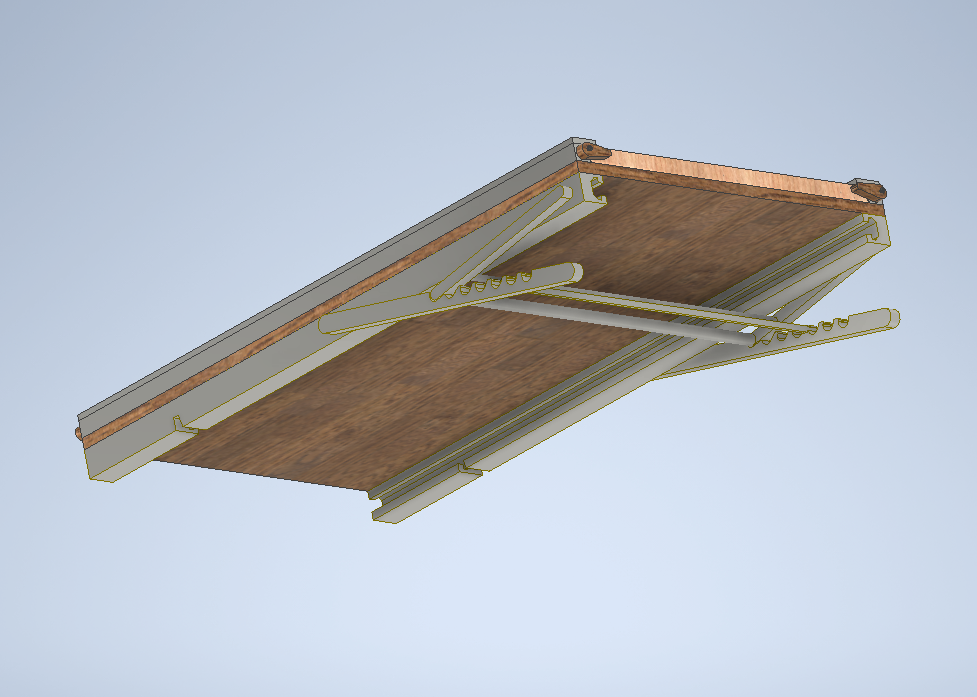
\includegraphics[width=\linewidth]{Bilder/Rampe_unten.png}
	\end{subfigure}
	\hfill
	\caption{Laufstegrampenkonstruktion mit zwei austauschbaren Platten und einer Winkelverstellung mit Raste. Links: Sicht von schräg oben mit eingeklappter Winkelverstellung. Rechts: Sicht von schräg unten mit niedigster Winkeleinstellung.}
	\label{Rampe_Inventor}
	%\vspace{0.1cm}
\end{figure}
Außerdem kann auf das MAP nur Einfluss genommen werden, wenn ein magnetisches Feld angelegt wird. Deshalb wurde ein Laufsteg mit einem Hohlraum angefertigt, um unter der Fläche, auf der NAO läuft, Magneten anzubringen. 

\begin{wrapfigure}{hr}{0.4\linewidth}
	\vspace{-0.5cm}
	\centering
	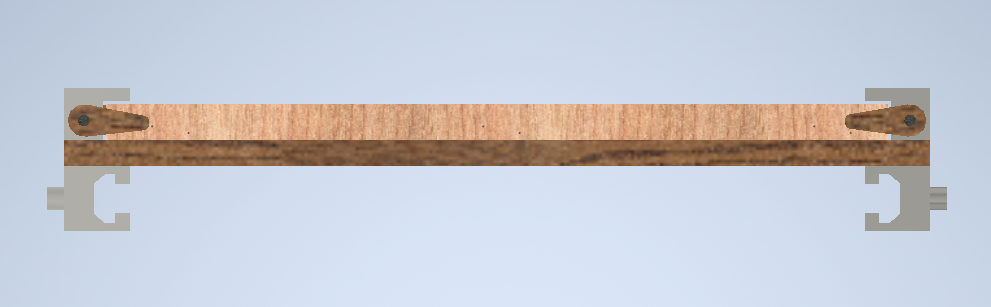
\includegraphics[width=\linewidth]{Bilder/Rampe_Seitenansicht3.png}
	\caption{Seitenansicht der Rampe mit einer Breite von $66,4 \unit{cm}$.}
	\label{Rampe_Seite_Inventor}
	\vspace{-0.5cm}
\end{wrapfigure}

% Aufbau der Rampe
Der Laufsteg besteht aus einer $120\times66,4 \unit{cm}$ großen Pressholzplatte, die auf der Oberseite mit einem Aluminiumkonstrukt erweitert ist, welches die Einschubplatten von beiden Längsseiten und nach oben hin abschließt, Abb. \ref{Rampe_Inventor} links. Auf den kurzen Seiten verriegeln jeweils zwei drehbare Keile den Einschub, sodass die Platten eingeschlossen werden, Abb. \ref{Rampe_Seite_Inventor}.

Auf der Unterseite sind an den Längsseiten zwei mit T-Nut versehene Aluminiumstangen angebracht, sowie eine zweiteilige Stangenkonstruktion, die eine Winkelverstellung mit Raste erlaubt, zu sehen in Abb. \ref{Rampe_Inventor} rechts. Die einstellbaren Winkel betragen ca. $5^\circ$ bis $17^\circ$, oder es wird für $0^\circ$ vollständig eingeklappt.
  
Man hat NAO bereits schräge Flächen gehen lassen wie in \cite{Lutz_naowalking}. Dies erfordert einen komplett anderen Gang und wäre über den zeitlichen Rahmen dieser Arbeit hinausgegangen. Die Neodymmagnete, die verwendet wurden, haben eine Haftkraft von ca. $16 \unit{kg}$, eine Maße von $40\times40\times4 \unit{mm}$ \cite{schraubmagnet} und wurden an die Unterseite der Rampe geschraubt. Die ersten Versuche ergaben schließlich, dass das MAP nur bei einem Abstand ohne Einlageplatten reagierte. Deshalb wurden in den gesamten Messungen ohne diese Platten durchgeführt. 

\FloatBarrier
% Was man für die Messungen verwendet hat

%\subsubsection{Genaueres zum Einsatz an dem Nao Roboter}

%%% Local Variables:
%%% mode: latex
%%% TeX-master: "main"
%%% End: